\chapter{Toegepaste statistische thermodynamica}\label{ch:b3:statistical-thermo-applied}

Vloeibare waterstof in de best geïsoleerde tank verdampt toch, en in de
eerste dagen na het vloeibaar maken verdampt ze veel sneller dan de warmte
die door de wanden lekt kan verklaren. De warmte komt uit de vloeistof
zelf. Waterstofmoleculen bestaan in twee vormen, die alleen verschillen in
de onderlinge oriëntatie van de spins van hun twee protonen en die maar
heel traag in elkaar overgaan; bij \qty{20}{K} komt bij de omzetting van de
ene vorm in de andere meer warmte vrij dan nodig is om de vloeistof te
verdampen. Dit hoofdstuk past de toestandssommen van
\cref{ch:b3:partition-functions} toe op warmtecapaciteiten, op deze
kernspinisomeren en op de entropie die sommige kristallen bij 0 K
behouden, en berekent daarna evenwichtsconstanten en isotoopeffecten
uitsluitend uit spectroscopische gegevens.

\begin{recall}
\Cref{ch:b3:partition-functions} bouwde de \omterm{def:b3:partition-functions:partition-function}{moleculaire toestandssom} en haar
vier factoren op, en leidde er $U$, $S$ en $G$ uit af. Het deel van jaar~2
verbond de standaardevenwichtsconstante met de standaardreactie-gibbsenergie,
$\Delta_rG^\circ = -RT\ln K^\circ$, en stelde de vergelijking van Van 't
Hoff op; \cref{ch:b3:many-electron-atoms} stelde dat een golffunctie van
teken verandert wanneer twee identieke fermionen verwisseld worden;
\cref{ch:b3:rovibrational-spectroscopy} vond de afwisseling 3:1 van de
lijnintensiteiten in het rotatieramanspectrum van moleculen zoals
\ce{H2}. Boek 1 (jaar 9) definieerde isotopen.
\end{recall}

\begin{omfigure}
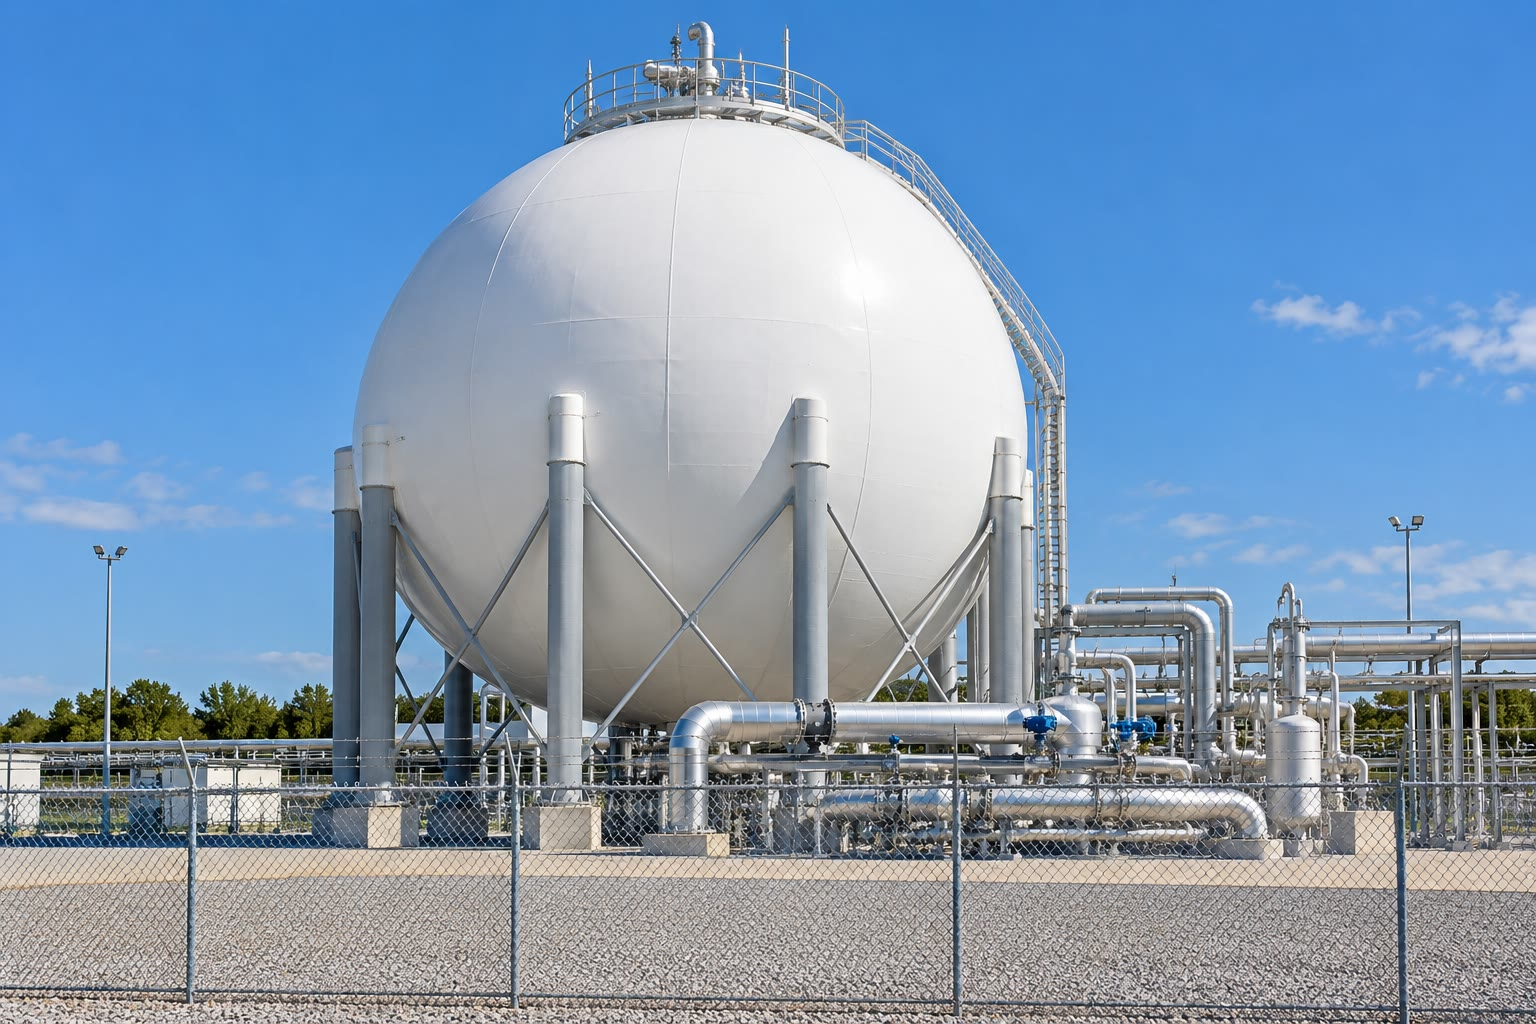
\includegraphics[width=0.6\linewidth]{images/book4/ai/b3-11-lh2-tank.jpg}

{\small Een bolvormige tank voor vloeibare waterstof. Bij \qty{20}{K} kan de
warmte die in de vloeistof ontstaat door de trage omzetting van de ene
kernspinvorm van waterstof in de andere, groter zijn dan de warmte die
van buiten binnenlekt.}
\end{omfigure}

\section{Warmtecapaciteiten van gassen}

De warmtecapaciteit bij constant volume is $C_V = (\partial U/\partial T)_V$, en met
\cref{thm:b3:partition-functions:internal-energy} draagt elk soort beweging
afzonderlijk bij. Twee limieten beheersen alles.

\begin{theorem}[Equipartitiestelling]\label{thm:b3:statistical-thermo-applied:equipartition}
Wanneer de energieniveaus van een beweging dicht bij elkaar liggen in
vergelijking met $kT$, draagt elke term van haar energie die kwadratisch
is in een coördinaat of een impuls
$\frac12kT$ bij tot de gemiddelde energie van een molecuul, en dus $\frac12R$ tot de
molaire warmtecapaciteit. Deze uitspraak is de
\emph{equipartitiestelling}\index{equipartitiestelling}.
\end{theorem}

\begin{proof}[Gedeeltelijk bewijs]
In de klassieke limiet wordt de som over de toestanden van een beweging
een integraal, en een kwadratische term $a u^2$ draagt de factor $\int\eu^{-\beta au^2}\dd u =
\sqrt{\pi/\beta a}$ bij, evenredig met $\beta^{-1/2}$. Volgens
\cref{thm:b3:partition-functions:internal-energy} is zijn gemiddelde energie
$-\partial\ln(\beta^{-1/2})/\partial\beta = 1/2\beta = \frac12kT$. Dat de
klassieke integraal de limiet is van de kwantumsom, werd voor translatie
en rotatie aangetoond in
\cref{ch:b3:partition-functions}; voor vibratie volgt het uit de volgende
propositie wanneer $T \gg \theta_{\mathrm V}$.
\end{proof}

Translatie heeft drie kwadratische termen ($\frac32R$); de rotatie van een
lineair molecuul twee ($R$), van een niet-lineair molecuul drie
($\frac32R$); elke vibratie twee, kinetisch en potentieel ($R$). Een
lineair molecuul met $N$ atomen nadert dus bij hoge temperatuur tot
$C_{V,\mathrm m} = \frac52R + (3N - 5)R$. Voor vibraties wordt de limiet
bij kamertemperatuur bijna nooit bereikt.

\begin{proposition}[Vibratiewarmtecapaciteit]\label{prop:b3:statistical-thermo-applied:cv-vib}
Een harmonische vibratie met karakteristieke temperatuur $\theta_{\mathrm V}$ levert, met
$x = \theta_{\mathrm V}/T$, de bijdrage
\[
  \frac{C_{V,\mathrm m}^{\mathrm V}}{R} = \frac{x^2\eu^x}{(\eu^x - 1)^2},
\]
de einsteinfunctie, die naar 1 gaat wanneer $T \gg \theta_{\mathrm V}$ en
exponentieel daalt, als $x^2\eu^{-x}$, wanneer $T \ll \theta_{\mathrm V}$.
\end{proposition}

\begin{proof}
Uit \cref{prop:b3:partition-functions:q-vib} volgt $U - U(0) = R\theta_{\mathrm V}/(\eu^x - 1)$ per mol.
Differentiëren naar $T$, met $\dd x/\dd T = -x/T$, geeft
$R\theta_{\mathrm V}\eu^x(x/T)/(\eu^x - 1)^2 = Rx^2\eu^x/(\eu^x - 1)^2$. Voor $x \to 0$ is $\eu^x - 1 \approx x$ en
gaat de verhouding naar 1; voor grote $x$ gedraagt ze zich als $x^2\eu^{-x}$.
\end{proof}

\begin{method}[De warmtecapaciteit van een gas uit zijn bewegingen]\label{met:b3:statistical-thermo-applied:cv}
\begin{enumerate}
  \item Translatie: altijd $\frac32R$.
  \item Rotatie: $R$ (lineair) of $\frac32R$ (niet-lineair) als $T \gg \theta_{\mathrm R}$, wat voor
        elk gas behalve waterstof geldt boven enkele tientallen kelvin.
  \item Vibraties: één einsteinterm per \omterm{def:b3:group-theory-applied:normal-mode}{normaaltrilling}, met $\theta_{\mathrm V} = hc\tilde\nu/k$ uit
        de fundamentele golfgetallen; een ontaarde trilling telt zo vaak
        mee als haar \omterm{def:b3:quantum-model-systems:degenerate}{ontaardingsgraad}.
  \item Tel op, en $C_{p,\mathrm m} = C_{V,\mathrm m} + R$ voor een ideaal gas.
\end{enumerate}
\end{method}

Men zegt dat een beweging bevroren is wanneer $kT$ klein is in vergelijking
met haar eerste excitatie: ze bevat dan geen energie en draagt niets bij
tot $C_V$. De vibratie van \ce{N2} ($\theta_{\mathrm V} = \qty{3352}{K}$) is
bij kamertemperatuur bevroren en
$C_{V,\mathrm m} = \frac52R$; die van \ce{Cl2} ($\theta_{\mathrm V} = \qty{798}{K}$) is half wakker,
$C_{V,\mathrm m} = 3.07R$ bij \qty{300}{K}.

\begin{omfigure}
\begin{tikzpicture}
\begin{axis}[width=0.86\linewidth, height=6.4cm, xmode=log, xmin=10, xmax=3000,
  ymin=1.3, ymax=3.9, axis lines=left, xlabel={$T$ / K}, ylabel={$C_{V,\mathrm m}/R$},
  tick label style={font=\small}, label style={font=\small},
  log ticks with fixed point, xtick={10,30,100,300,1000,3000},
  unbounded coords=jump]
\addplot[omDef, thick] table[x=T, y=N2] {figdata/out/bachelor-3-heat-capacity.dat};
\addplot[black!60, thick] table[x=T, y=Cl2] {figdata/out/bachelor-3-heat-capacity.dat};
\addplot[omThm, thick, dashed] table[x=T, y=nH2] {figdata/out/bachelor-3-heat-capacity.dat};
\addplot[omThm, thick] table[x=T, y=eH2] {figdata/out/bachelor-3-heat-capacity.dat};
\addplot[only marks, mark=*, mark size=1.6pt, omDef] table[x=T, y=N2] {figdata/out/bachelor-3-heat-capacity-janaf.dat};
\addplot[only marks, mark=square*, mark size=1.5pt, black!60] table[x=T, y=Cl2] {figdata/out/bachelor-3-heat-capacity-janaf.dat};
\draw[black!30, densely dotted] (axis cs:10,1.5) -- (axis cs:3000,1.5);
\draw[black!30, densely dotted] (axis cs:10,2.5) -- (axis cs:3000,2.5);
\draw[black!30, densely dotted] (axis cs:10,3.5) -- (axis cs:3000,3.5);
\node[font=\scriptsize, black!60, anchor=south east] at (axis cs:2900,1.5) {$\frac32$: translatie};
\node[font=\scriptsize, black!60, anchor=south west] at (axis cs:10.5,2.5) {$\frac52$: + rotatie};
\node[font=\scriptsize, black!60, anchor=south west] at (axis cs:10.5,3.5) {$\frac72$: + vibratie};
\node[font=\scriptsize, omThm, anchor=south west] at (axis cs:60,3.6) {\ce{H2} in evenwicht};
\node[font=\scriptsize, omThm, anchor=north west] at (axis cs:130,1.78) {normaal \ce{H2}};
\node[font=\scriptsize, black!70, anchor=south east] at (axis cs:560,3.33) {\ce{Cl2}};
\node[font=\scriptsize, omDef, anchor=south east] at (axis cs:1000,3.0) {\ce{N2}};
\end{axis}
\end{tikzpicture}

{\small Molaire warmtecapaciteit bij constant volume, berekend uit de
spectroscopische constanten (lijnen; \omterm{def:b3:quantum-model-systems:rotor}{starre rotor}, harmonische vibratie),
met de waarden van de thermochemische tabellen voor \ce{N2} en \ce{Cl2}
(punten, $C_p/R - 1$). De vibratie ontwaakt rond $\theta_{\mathrm V}/10$;
boven ongeveer \qty{1000}{K} stijgen de tabellen boven het harmonische
model, dat de anharmoniciteit mist. Waterstof: de rotatiebijdrage van
normale waterstof (gestreept, ortho en para bevroren in de verhouding 3:1)
en van waterstof in evenwicht (doorgetrokken), die boven $\frac52$
uitschiet omdat de omzetting van para in ortho warmte opneemt.}
\end{omfigure}

\section{Kernspinstatistiek}

De twee kernen van \ce{H2} zijn identieke fermionen. Ze verwisselen
verandert het teken van de totale golffunctie
(\cref{ch:b3:many-electron-atoms}); ze verwisselen is hetzelfde als het
molecuul kop over staart draaien, wat de rotatiegolffunctie $Y_{J,M}$ met
$(-1)^J$ vermenigvuldigt en de kernspinfunctie met $+1$ of $-1$.

\begin{theorem}[Kernspinstatistiek]\label{thm:b3:statistical-thermo-applied:spin-statistics}
In een homonucleair diatomisch molecuul waarvan de kernen spin $I$ hebben,
in een elektronische grondtoestand ${}^1\Sigma_g^+$, zijn er $(2I+1)(I+1)$
symmetrische en $(2I+1)I$ antisymmetrische kernspintoestanden. Voor
fermionen (halftallige $I$) horen de antisymmetrische bij even $J$ en de
symmetrische bij oneven $J$; voor bosonen (gehele $I$) is het omgekeerd.
Voor \ce{H2} ($I = \frac12$) hebben even en oneven niveaus de spingewichten
1 en 3; voor \ce{D2} ($I = 1$) 6 en 3. Als $I = 0$ bestaat er maar één
pariteit van $J$: het lineaire \ce{CO2}-molecuul, met twee
\ce{^{16}O}-kernen en een symmetrische grondtoestand, heeft alleen even
rotatieniveaus.
\end{theorem}

\begin{proof}[Gedeeltelijk bewijs]
Het symmetriepostulaat (de totale golffunctie is antisymmetrisch onder
verwisseling van twee identieke fermionen, symmetrisch voor bosonen) wordt
aangenomen. De $(2I+1)^2$ producten van spintoestanden van één kern
$|m_1\rangle|m_2\rangle$ geven $2I+1$ symmetrische toestanden met $m_1 = m_2$,
en voor elk van de $(2I+1)2I/2$ paren $m_1 \ne m_2$ één symmetrische en één
antisymmetrische combinatie: $(2I+1) + (2I+1)I = (2I+1)(I+1)$
symmetrische en $(2I+1)I$ antisymmetrische toestanden. In een toestand
${}^1\Sigma_g^+$ blijven de elektronische en vibratiefuncties onveranderd
bij de verwisseling, zodat het product van rotatie- en spinfuncties het
vereiste totale teken moet hebben: voor fermionen is
$(-1)^J \times(\text{spinsymmetrie}) = -1$, wat even $J$ koppelt aan
antisymmetrische spintoestanden. Voor \ce{H2}: 3 symmetrische, 1
antisymmetrische; voor \ce{D2}: 6 en
3.
\end{proof}

\begin{definition}[Ortho- en parawaterstof]\label{def:b3:statistical-thermo-applied:spin-isomers}
\emph{Orthowaterstof}\index{orthowaterstof} is de vorm van \ce{H2} waarin de
twee protonspins zich in een symmetrische toestand (triplet) bevinden, en
die alleen de oneven rotatieniveaus bezet;
\emph{parawaterstof}\index{parawaterstof} is de vorm met de
antisymmetrische spintoestand (singulet), die alleen de even niveaus bezet.
\end{definition}

De ene vorm in de andere omzetten vereist dat één kernspin ten opzichte
van de andere omklapt, wat botsingen met andere waterstofmoleculen
nauwelijks bewerkstelligen: in zuivere waterstof gedragen de twee vormen
zich dagenlang als twee verschillende gassen. Een paramagnetisch
oppervlak, waarvan het inhomogene magneetveld verschillend inwerkt op de
twee protonen, katalyseert de omzetting.

\begin{proposition}[Evenwichtsverhouding ortho-para]\label{prop:b3:statistical-thermo-applied:ortho-para}
In evenwicht is de fractie \omterm{def:b3:statistical-thermo-applied:spin-isomers}{parawaterstof}
\[
  x_{\mathrm{para}} = \frac{\sum_{J\,\mathrm{even}}(2J+1)\eu^{-\theta_{\mathrm R}J(J+1)/T}}
    {\sum_{J\,\mathrm{even}}(2J+1)\eu^{-\theta_{\mathrm R}J(J+1)/T} + 3\sum_{J\,\mathrm{oneven}}(2J+1)\eu^{-\theta_{\mathrm R}J(J+1)/T}},
\]
die naar 1 gaat bij 0 K en naar $\frac14$ bij hoge temperatuur. Voor
\ce{D2} gaat de orthovorm
(even $J$) naar 1 bij 0 K en naar $\frac23$ bij hoge temperatuur.
\end{proposition}

\begin{proof}
De \omterm{def:b3:partition-functions:boltzmann}{boltzmannverdeling} over alle toestanden, met de spingewichten van
\cref{thm:b3:statistical-thermo-applied:spin-statistics}. Bij 0 K is
alleen $J = 0$, dat even is, bezet. Bij hoge temperatuur zijn de even en
de oneven som elk de helft van $T/\theta_{\mathrm R}$, en is de verhouding
$1 : 3$; voor \ce{D2} $6 : 3$.
\end{proof}

Voor \ce{H2} is $\theta_{\mathrm R} = \qty{85.4}{K}$: het mengsel in evenwicht is voor de helft para bij \qty{78}{K},
voor 99.8\,\% para bij het kookpunt, \qty{20.37}{K}, en voor 25.07\,\% bij
kamertemperatuur. Waterstof die bij kamertemperatuur bewaard wordt,
normale waterstof genoemd, is dus een mengsel van ortho en para in de
verhouding 3:1.

\begin{omfigure}
\begin{tikzpicture}
\begin{axis}[width=0.72\linewidth, height=5.4cm, xmin=0, xmax=300, ymin=0, ymax=1.05,
  axis lines=left, xlabel={$T$ / K}, ylabel={fractie in evenwicht},
  tick label style={font=\small}, label style={font=\small}]
\addplot[omThm, thick] table[x=T, y=pH2] {figdata/out/bachelor-3-ortho-para.dat};
\addplot[omDef, thick] table[x=T, y=oD2] {figdata/out/bachelor-3-ortho-para.dat};
\draw[black!35, densely dotted] (axis cs:0,0.25) -- (axis cs:300,0.25);
\draw[black!35, densely dotted] (axis cs:0,0.6667) -- (axis cs:300,0.6667);
\node[font=\scriptsize, omThm, anchor=south west] at (axis cs:190,0.27) {parafractie van \ce{H2} $\to \frac14$};
\node[font=\scriptsize, omDef, anchor=south west] at (axis cs:120,0.69) {orthofractie van \ce{D2} $\to \frac23$};
\end{axis}
\end{tikzpicture}

{\small Evenwichtssamenstelling van de kernspinisomeren als functie van de
temperatuur, uit de rotatieniveaus en de spingewichten (\ce{H2}: 1 en 3;
\ce{D2}: 6 en 3). Bij lage temperatuur krijgen beide vormen met even $J$
de overhand.}
\end{omfigure}

De warmtecapaciteit van waterstof toont de gevolgen. In normale waterstof
zijn de ortho- en paramoleculen twee gassen die in vaste verhoudingen
gemengd zijn; elk heeft zijn eigen ladder van niveaus, die begint bij
$J = 1$ en bij $J = 0$, en zijn rotatie bevriest afzonderlijk. In waterstof
in evenwicht zet het opwarmen ook para om in ortho, wat energie opneemt en
de piek van de figuur hierboven geeft. De eerste metingen, zonder
katalysator uitgevoerd, volgden de kromme van normale waterstof, en het
was de interpretatie van die kromme als een bevroren mengsel 3:1 die de
twee vormen voor het eerst aan het licht bracht.

\begin{remark}
Het \omterm{def:b3:partition-functions:symmetry-number}{symmetriegetal} van \cref{prop:b3:partition-functions:q-rot} is nu
verantwoord. Bij hoge temperatuur vindt elke spintoestand ongeveer de
helft van de rotatieniveaus toegestaan, zodat $\sum(\text{spingewicht})(2J+1)\eu^{\dots} \approx (2I+1)^2\,T/2\theta_{\mathrm R}$: de
totale spinfactor $(2I+1)^2$ wordt volgens afspraak weggelaten, en $\sigma = 2$ blijft over.
\end{remark}

\begin{definition}[Restentropie]\label{def:b3:statistical-thermo-applied:residual-entropy}
De \emph{restentropie}\index{restentropie} van een kristal is de entropie
die het behoudt wanneer $T \to 0$, omdat zijn moleculen bevroren blijven in
een van vele schikkingen met dezelfde of bijna dezelfde energie.
\end{definition}

\begin{proposition}[Restentropie van koolstofmonoxide en van ijs]\label{prop:b3:statistical-thermo-applied:residual}
Een kristal van $N$ moleculen dat bevroren is in $W_0$ even waarschijnlijke
schikkingen heeft $S_0 =
k\ln W_0$. Vast \ce{CO}, waarin elk molecuul in twee richtingen kan
wijzen, heeft $S_{0,\mathrm m} = R\ln2 =
\qty{5.76}{J.K^{-1}.mol^{-1}}$. IJs, waarin elk zuurstofatoom aan twee
waterstofatomen gebonden is en via waterstofbruggen aan twee andere, heeft
$W_0 = (3/2)^N$ en $S_{0,\mathrm m} = R\ln\frac32 =
\qty{3.37}{J.K^{-1}.mol^{-1}}$.
\end{proposition}

\begin{proof}
\cref{def:b3:partition-functions:statistical-entropy} toegepast bij $T \to 0$.
\ce{CO}: de dipool van het molecuul is zo klein dat de oriëntaties CO en OC
bijna dezelfde energie hebben, en elk van de $N$ moleculen heeft er twee: $W_0 = 2^N$,
$S_0 = Nk\ln2$. IJs (de telling van Pauling): elk van de $2N$
waterstofatomen zit op een lijn O$\cdots$O, dicht bij het ene of het andere
uiteinde: $2^{2N}$ schikkingen. Van de 16 manieren om de vier
waterstofatomen rond één zuurstofatoom te plaatsen, geven er 6 precies twee
nabije waterstofatomen (een watermolecuul); als de zuurstofatomen als
onafhankelijk behandeld worden, voldoet een fractie
$6/16$ van de schikkingen aan elk ervan: $W_0 = 2^{2N}(6/16)^N = (3/2)^N$.
\end{proof}

De tabellen vermelden voor \ce{CO} de \omterm{def:b3:partition-functions:statistical-entropy}{statistische entropie}
(\cref{ch:b3:partition-functions}); de calorimetrische waarde ligt lager,
met een verschil van de orde van $R\ln2$, iets kleiner omdat de
oriëntaties niet helemaal willekeurig zijn. Voor ijs stemde het verschil
tussen de calorimetrische entropie van waterdamp en haar statistische
waarde overeen met de telling van Pauling toen hij die in 1935 maakte, wat
bevestigde dat de protonen van ijs wanordelijk zijn. De derde hoofdwet,
in de vorm ``de entropie van een perfect kristal is nul bij 0 K'', geldt
voor de kristallen die wel één enkele schikking bereiken.

\begin{omfigure}
\begin{tikzpicture}[scale=1.15, every node/.style={transform shape}]
  \draw[black!45, dashed] (0.00,0.00) -- (1.20,0.00);
  \draw[black, thick] (0.00,0.00) -- (0.36,0.00); \node[aH, minimum size=2.2mm] at (0.36,0.00) {};
  \draw[black!45, dashed] (0.00,0.00) -- (0.00,1.20);
  \draw[black, thick] (0.00,0.00) -- (0.00,0.36); \node[aH, minimum size=2.2mm] at (0.00,0.36) {};
  \draw[black!45, dashed] (0.00,1.20) -- (1.20,1.20);
  \draw[black, thick] (0.00,1.20) -- (0.36,1.20); \node[aH, minimum size=2.2mm] at (0.36,1.20) {};
  \draw[black!45, dashed] (0.00,1.20) -- (0.00,2.40);
  \draw[black, thick] (0.00,2.40) -- (0.00,2.04); \node[aH, minimum size=2.2mm] at (0.00,2.04) {};
  \draw[black!45, dashed] (0.00,2.40) -- (1.20,2.40);
  \draw[black, thick] (1.20,2.40) -- (0.84,2.40); \node[aH, minimum size=2.2mm] at (0.84,2.40) {};
  \draw[black!45, dashed] (0.00,2.40) -- (0.00,3.60);
  \draw[black, thick] (0.00,3.60) -- (0.00,3.24); \node[aH, minimum size=2.2mm] at (0.00,3.24) {};
  \draw[black!45, dashed] (0.00,3.60) -- (1.20,3.60);
  \draw[black, thick] (1.20,3.60) -- (0.84,3.60); \node[aH, minimum size=2.2mm] at (0.84,3.60) {};
  \draw[black!45, dashed] (0.00,3.60) -- (0.00,4.20);
  \draw[black, thick] (0.00,3.60) -- (0.00,3.96); \node[aH, minimum size=2.2mm] at (0.00,3.96) {};
  \draw[black!45, dashed] (1.20,0.00) -- (2.40,0.00);
  \draw[black, thick] (1.20,0.00) -- (1.56,0.00); \node[aH, minimum size=2.2mm] at (1.56,0.00) {};
  \draw[black!45, dashed] (1.20,0.00) -- (1.20,1.20);
  \draw[black, thick] (1.20,1.20) -- (1.20,0.84); \node[aH, minimum size=2.2mm] at (1.20,0.84) {};
  \draw[black!45, dashed] (1.20,1.20) -- (2.40,1.20);
  \draw[black, thick] (2.40,1.20) -- (2.04,1.20); \node[aH, minimum size=2.2mm] at (2.04,1.20) {};
  \draw[black!45, dashed] (1.20,1.20) -- (1.20,2.40);
  \draw[black, thick] (1.20,1.20) -- (1.20,1.56); \node[aH, minimum size=2.2mm] at (1.20,1.56) {};
  \draw[black!45, dashed] (1.20,2.40) -- (2.40,2.40);
  \draw[black, thick] (1.20,2.40) -- (1.56,2.40); \node[aH, minimum size=2.2mm] at (1.56,2.40) {};
  \draw[black!45, dashed] (1.20,2.40) -- (1.20,3.60);
  \draw[black, thick] (1.20,3.60) -- (1.20,3.24); \node[aH, minimum size=2.2mm] at (1.20,3.24) {};
  \draw[black!45, dashed] (1.20,3.60) -- (2.40,3.60);
  \draw[black, thick] (2.40,3.60) -- (2.04,3.60); \node[aH, minimum size=2.2mm] at (2.04,3.60) {};
  \draw[black!45, dashed] (1.20,3.60) -- (1.20,4.20);
  \draw[black!45, dashed] (2.40,0.00) -- (3.60,0.00);
  \draw[black, thick] (3.60,0.00) -- (3.24,0.00); \node[aH, minimum size=2.2mm] at (3.24,0.00) {};
  \draw[black!45, dashed] (2.40,0.00) -- (2.40,1.20);
  \draw[black, thick] (2.40,0.00) -- (2.40,0.36); \node[aH, minimum size=2.2mm] at (2.40,0.36) {};
  \draw[black!45, dashed] (2.40,1.20) -- (3.60,1.20);
  \draw[black, thick] (2.40,1.20) -- (2.76,1.20); \node[aH, minimum size=2.2mm] at (2.76,1.20) {};
  \draw[black!45, dashed] (2.40,1.20) -- (2.40,2.40);
  \draw[black, thick] (2.40,2.40) -- (2.40,2.04); \node[aH, minimum size=2.2mm] at (2.40,2.04) {};
  \draw[black!45, dashed] (2.40,2.40) -- (3.60,2.40);
  \draw[black, thick] (3.60,2.40) -- (3.24,2.40); \node[aH, minimum size=2.2mm] at (3.24,2.40) {};
  \draw[black!45, dashed] (2.40,2.40) -- (2.40,3.60);
  \draw[black, thick] (2.40,2.40) -- (2.40,2.76); \node[aH, minimum size=2.2mm] at (2.40,2.76) {};
  \draw[black!45, dashed] (2.40,3.60) -- (3.60,3.60);
  \draw[black, thick] (2.40,3.60) -- (2.76,3.60); \node[aH, minimum size=2.2mm] at (2.76,3.60) {};
  \draw[black!45, dashed] (2.40,3.60) -- (2.40,4.20);
  \draw[black!45, dashed] (3.60,0.00) -- (4.20,0.00);
  \draw[black, thick] (3.60,0.00) -- (3.96,0.00); \node[aH, minimum size=2.2mm] at (3.96,0.00) {};
  \draw[black!45, dashed] (3.60,0.00) -- (3.60,1.20);
  \draw[black, thick] (3.60,1.20) -- (3.60,0.84); \node[aH, minimum size=2.2mm] at (3.60,0.84) {};
  \draw[black!45, dashed] (3.60,1.20) -- (4.20,1.20);
  \draw[black!45, dashed] (3.60,1.20) -- (3.60,2.40);
  \draw[black, thick] (3.60,1.20) -- (3.60,1.56); \node[aH, minimum size=2.2mm] at (3.60,1.56) {};
  \draw[black!45, dashed] (3.60,2.40) -- (4.20,2.40);
  \draw[black!45, dashed] (3.60,2.40) -- (3.60,3.60);
  \draw[black, thick] (3.60,2.40) -- (3.60,2.76); \node[aH, minimum size=2.2mm] at (3.60,2.76) {};
  \draw[black!45, dashed] (3.60,3.60) -- (4.20,3.60);
  \draw[black, thick] (3.60,3.60) -- (3.96,3.60); \node[aH, minimum size=2.2mm] at (3.96,3.60) {};
  \draw[black!45, dashed] (3.60,3.60) -- (3.60,4.20);
  \draw[black, thick] (3.60,3.60) -- (3.60,3.96); \node[aH, minimum size=2.2mm] at (3.60,3.96) {};
  \draw[black!45, dashed] (-0.60,0.00) -- (0.00,0.00);
  \draw[black!45, dashed] (-0.60,1.20) -- (0.00,1.20);
  \draw[black, thick] (0.00,1.20) -- (-0.36,1.20); \node[aH, minimum size=2.2mm] at (-0.36,1.20) {};
  \draw[black!45, dashed] (-0.60,2.40) -- (0.00,2.40);
  \draw[black, thick] (0.00,2.40) -- (-0.36,2.40); \node[aH, minimum size=2.2mm] at (-0.36,2.40) {};
  \draw[black!45, dashed] (-0.60,3.60) -- (0.00,3.60);
  \draw[black!45, dashed] (0.00,-0.60) -- (0.00,0.00);
  \draw[black!45, dashed] (1.20,-0.60) -- (1.20,0.00);
  \draw[black, thick] (1.20,0.00) -- (1.20,-0.36); \node[aH, minimum size=2.2mm] at (1.20,-0.36) {};
  \draw[black!45, dashed] (2.40,-0.60) -- (2.40,0.00);
  \draw[black, thick] (2.40,0.00) -- (2.40,-0.36); \node[aH, minimum size=2.2mm] at (2.40,-0.36) {};
  \draw[black!45, dashed] (3.60,-0.60) -- (3.60,0.00);
  \node[aO, minimum size=4mm] at (0.00,0.00) {};
  \node[aO, minimum size=4mm] at (0.00,1.20) {};
  \node[aO, minimum size=4mm] at (0.00,2.40) {};
  \node[aO, minimum size=4mm] at (0.00,3.60) {};
  \node[aO, minimum size=4mm] at (1.20,0.00) {};
  \node[aO, minimum size=4mm] at (1.20,1.20) {};
  \node[aO, minimum size=4mm] at (1.20,2.40) {};
  \node[aO, minimum size=4mm] at (1.20,3.60) {};
  \node[aO, minimum size=4mm] at (2.40,0.00) {};
  \node[aO, minimum size=4mm] at (2.40,1.20) {};
  \node[aO, minimum size=4mm] at (2.40,2.40) {};
  \node[aO, minimum size=4mm] at (2.40,3.60) {};
  \node[aO, minimum size=4mm] at (3.60,0.00) {};
  \node[aO, minimum size=4mm] at (3.60,1.20) {};
  \node[aO, minimum size=4mm] at (3.60,2.40) {};
  \node[aO, minimum size=4mm] at (3.60,3.60) {};
\end{tikzpicture}

{\small Protonenwanorde in ijs, getekend als een vlak vierkant netwerk (het
echte netwerk is tetraëdrisch): elk zuurstofatoom (rood) heeft vier buren
O$\cdots$O, één waterstofatoom (wit) op elke lijn, en precies twee
waterstofatomen dicht bij zich (de ijsregels). Dit is een van de $(3/2)^N$
schikkingen van de telling van Pauling; ze hebben alle bijna dezelfde
energie, en bevriezen kiest er willekeurig één uit.}
\end{omfigure}

\section{Evenwichtsconstanten uit toestandssommen}

\begin{theorem}[Evenwichtsconstante uit toestandssommen]\label{thm:b3:statistical-thermo-applied:k-from-q}
Voor een reactie $0 = \sum_J\nu_J\mathrm J$ tussen ideale gassen is
\[
  K^\circ = \prod_J\Bigl(\frac{q^\circ_{J,\mathrm m}}{N_A}\Bigr)^{\nu_J}\eu^{-\Delta_rE_0/RT},
\]
waarin $q^\circ_{J,\mathrm m}$ de toestandssom van $\mathrm J$ is in het
standaard molair volume
$V^\circ_{\mathrm m} = RT/p^\circ$, elk geteld vanaf zijn eigen
grondtoestand, en $\Delta_rE_0 =
\sum\nu_JE_{0,J}$ de molaire reactie-energie bij 0 K is, van de
grondtoestand van de beginstoffen naar die van de producten.
\end{theorem}

\begin{proof}
Volgens \cref{thm:b3:partition-functions:entropy} heeft een mol ideaal gas $\mathrm J$ bij $p^\circ$
$G^\circ_{\mathrm m} - G_{\mathrm m}(0) = -RT\ln(q^\circ_{J,\mathrm m}/N_A)$, en $G_{\mathrm m}(0)$ is de energie $E_{0,J}$
van zijn grondtoestand op een schaal die alle deeltjes gemeen hebben. Dus
is $\Delta_rG^\circ =
\Delta_rE_0 - RT\sum_J\nu_J\ln(q^\circ_{J,\mathrm m}/N_A)$, en $\Delta_rG^\circ = -RT\ln K^\circ$ geeft het
resultaat.
\end{proof}

\begin{method}[Een evenwichtsconstante berekenen uit spectroscopische gegevens]\label{met:b3:statistical-thermo-applied:k-stat}
\begin{enumerate}
  \item Voor elk deeltje: $q^\circ_{\mathrm m}/N_A = (kT/p^\circ)\Lambda^{-3}\times q^{\mathrm R}q^{\mathrm V}q^{\mathrm E}$, met
        symmetriegetallen en elektronische ontaardingsgraden.
  \item $\Delta_rE_0$ uit dissociatie-energieën $D_0$ (gemeten vanaf het
        laagste vibratieniveau, zodat de nulpuntsenergieën inbegrepen zijn)
        of uit vormingsenthalpieën bij 0 K.
  \item Vermenigvuldig, en controleer de eenheden: $K^\circ$ is een zuiver
        getal, waarbij de standaarddruk binnenkomt via $kT/p^\circ$.
\end{enumerate}
\end{method}

\begin{example}[De dissociatie van jood]\label{ex:b3:statistical-thermo-applied:iodine}
% ledger: janaf:I.dfH0, janaf:I2g.dfH0, lev:I.2P1_2, diat:I2.we, diat:I2.wexe, diat:I2.Be, diat:I2.ae, aw:I, janaf:I.logKf.1000
Voor $\ce{I2(g) <=> 2 I(g)}$ is $\Delta_rE_0 = D_0(\ce{I2}) = 2 \times 107.164 - 65.504 = \qty{148.824}{kJ/mol}$,
uit de vormingsenthalpieën bij 0 K van de thermochemische tabellen. Bij
\qty{1000}{K}: voor I is $\Lambda = \qty{4.90}{pm}$, $kT/p^\circ = \qty{1.381e-25}{m^3}$, $q^{\mathrm E} = 4 +
2\eu^{-10.94} = 4.0000$ (het niveau ${}^2P_{1/2}$ ligt \qty{7603}{cm^{-1}}
hoger), dus $q^\circ_{\mathrm m}/N_A = \num{4.69e9}$;
voor \ce{I2} is $\Lambda = \qty{3.47}{pm}$, $q^{\mathrm R} = 1000/(2 \times 0.05369) = 9313$ en $q^{\mathrm V} = 3.784$, dus
$q^\circ_{\mathrm m}/N_A = \num{1.17e14}$. Dan is $K^\circ = (4.69\times10^9)^2/(1.17\times10^{14}) \times \eu^{-17.90} =
\num{3.17e-3}$, $\log K^\circ = -2.50$; de tabellen geven $-2.51$.
\end{example}

\begin{omfigure}
\begin{tikzpicture}
\begin{axis}[name=ki, width=0.5\linewidth, height=5.6cm, xmin=0.58, xmax=1.45, ymin=-6.5,
  ymax=1, axis lines=left, xlabel={$1000\,\mathrm K/T$}, ylabel={$\log K^\circ$},
  tick label style={font=\small}, label style={font=\small},
  title={\small $\ce{I2 <=> 2 I}$}]
\addplot[black, thick] table[x=invT, y=logK] {figdata/out/bachelor-3-equilibrium-constant-stat-i2.dat};
\addplot[only marks, mark=*, mark size=1.8pt, omThm] table[x=invT, y=logK] {figdata/out/bachelor-3-equilibrium-constant-stat-i2-janaf.dat};
\node[font=\scriptsize, anchor=north east, align=right] at (axis cs:1.43,0.8) {lijn: statistisch\\ punten: tabellen};
\end{axis}
\begin{axis}[at={(ki.east)}, anchor=west, xshift=1.4cm, width=0.44\linewidth, height=5.6cm,
  xmin=0, xmax=2000, ymin=0, ymax=4.4, axis lines=left, xlabel={$T$ / K},
  ylabel={$K^\circ$}, tick label style={font=\small}, label style={font=\small},
  title={\small $\ce{H2 + D2 <=> 2 HD}$}, scaled x ticks=false,
  xticklabel style={/pgf/number format/1000 sep={}}]
\addplot[omDef, thick] table[x=T, y=K] {figdata/out/bachelor-3-equilibrium-constant-stat-hd.dat};
\draw[black!35, densely dotted] (axis cs:0,4) -- (axis cs:2000,4);
\node[font=\scriptsize, anchor=north east] at (axis cs:1950,3.95) {limiet door $\sigma$: 4};
\end{axis}
\end{tikzpicture}

{\small Evenwichtsconstanten berekend uit toestandssommen. Links: de
dissociatie van jood, een rechte van Van 't Hoff met helling $-\Delta_rH^\circ/(R\ln10)$, met
de waarden van de thermochemische tabellen (punten). Rechts: de
uitwisseling $\ce{H2 + D2
<=> 2 HD}$, die bij hoge temperatuur nadert tot de verhouding van de
symmetriegetallen, 4, en bij lage temperatuur daaronder zakt door de
nulpuntsenergieën en de kernspinbeperkingen.}
\end{omfigure}

\begin{proposition}[De uitwisseling H$_2$ + D$_2$]\label{prop:b3:statistical-thermo-applied:hd}
Voor $\ce{H2 + D2 <=> 2 HD}$ gaat $K^\circ \to 4$ bij hoge temperatuur.
\end{proposition}

\begin{proof}
Bij hoge temperatuur zijn de translatie-, rotatie- en vibratiefactoren
$m^{3/2}$, $T/\sigma\theta_{\mathrm R} \propto \mu/\sigma$ en $T/\theta_{\mathrm V} \propto \sqrt\mu$ (de
\omterm{def:b3:quantum-model-systems:oscillator}{krachtconstante}, een elektronische eigenschap, is dezelfde voor de drie
moleculen), en $\Delta_rE_0/RT \to 0$.
Met $m_{\ce{H2}} = 2$, $m_{\ce{D2}} = 4$, $m_{\ce{HD}} = 3$ en $\mu = 1/2$, 1, $2/3$ (in eenheden van de
protonmassa, met verwaarlozing van het kleine verschil tussen D en 2H):
\[
  K^\circ \to \Bigl(\frac{9}{8}\Bigr)^{3/2} \times \frac{(2/3)^2/1^2}{(1/2)(1)/(2 \times 2)}
  \times \frac{2/3}{\sqrt{1/2}\sqrt1}
  = \frac{27}{16\sqrt2} \times \frac{32}{9} \times \frac{2\sqrt2}{3} = 4 .
\]
Alle massafactoren vallen precies weg: alleen de symmetriegetallen blijven
over, $\sigma_{\ce{H2}}
\sigma_{\ce{D2}}/\sigma_{\ce{HD}}^2 = 4$.
\end{proof}

Bij \qty{298.15}{K} bedraagt de statistische constante 3.26; de
nulpuntsenergieën van \ce{H2},
\ce{D2} en HD (\qty{2170.3}{cm^{-1}}, \qty{1542.3}{cm^{-1}} en \qty{1883.7}{cm^{-1}}) geven $\Delta_rE_0 =
\qty{54.8}{cm^{-1}}$, een factor $\eu^{-54.8/207.2} = 0.77$; de rotatie, die
voor deze lichte moleculen nog gedeeltelijk gekwantiseerd is, speelt ook
mee.

\begin{proposition}[De vergelijking van Van 't Hoff teruggevonden]\label{prop:b3:statistical-thermo-applied:vant-hoff-stat}
De statistische evenwichtsconstante voldoet aan $\dfrac{\dd\ln K^\circ}{\dd T} = \dfrac{\Delta_rH^\circ}{RT^2}$.
\end{proposition}

\begin{proof}
Elke $q^\circ_{J,\mathrm m}$ hangt van $T$ af via zijn niveaus en via $V^\circ_{\mathrm m} = RT/p^\circ$:
$\dd\ln q^\circ_{J,\mathrm m}/\dd T = (U_J - U_J(0))/RT^2 + 1/T$ per mol, volgens
\cref{thm:b3:partition-functions:internal-energy}. Dus is $\dd\ln K^\circ/\dd T =
[\Delta_rE_0 + \sum\nu_J(U_J - U_J(0)) + \sum\nu_JRT]/RT^2 = (\Delta_rU + \Delta\nu_{\mathrm g}RT)/RT^2 =
\Delta_rH^\circ/RT^2$ voor ideale gassen.
\end{proof}

Uit de helling van het linkerdeel van de figuur is de
dissociatie-enthalpie van jood rond \qty{1000}{K} gelijk aan
\qty{154}{kJ/mol}: $D_0$ plus de extra translatie-energie van twee atomen
ten opzichte van één molecuul, min zijn rotatie- en vibratie-energie.

\section{Isotoopeffecten}

\omterm{def:b3:rovibrational-spectroscopy:rotational-constant}{Isotopologen} hebben dezelfde elektronenstructuur, en dus dezelfde
potentiële-energiekromme en dezelfde \omterm{def:b3:quantum-model-systems:oscillator}{krachtconstanten}, maar verschillende
massa's: hun vibratiegolfgetallen, nulpuntsenergieën en toestandssommen
verschillen, en dus ook hun evenwichtsconstanten.

\begin{definition}[Evenwichtsisotoopeffect, fractioneringsfactor, $\delta$-waarde]\label{def:b3:statistical-thermo-applied:isotope-effect}
Het \emph{evenwichtsisotoopeffect}\index{evenwichtsisotoopeffect} van een
reactie is de verhouding $K_{\mathrm{licht}}/K_{\mathrm{zwaar}}$ van haar
evenwichtsconstanten met het lichte en het zware isotoop. De
\emph{fractioneringsfactor}\index{fractioneringsfactor}
tussen twee fasen of verbindingen A en B is $\alpha_{\mathrm{A/B}} = R_{\mathrm A}/R_{\mathrm B}$, waarin
$R$ de verhouding is van het zware tot het lichte isotoop (bijvoorbeeld
$\ce{^{18}O}/\ce{^{16}O}$). De
\emph{$\delta$-waarde}\index{delta-waarde@$\delta$-waarde} van een monster is $\delta = (R_{\mathrm{monster}}/R_{\mathrm{standaard}}
- 1) \times 1000$, in promille (\textperthousand).
\end{definition}

\begin{proposition}[Isotoopeffecten uit nulpuntsenergieën]\label{prop:b3:statistical-thermo-applied:zpe-isotope}
Voor een uitwisseling $\ce{XH + YD <=> XD + YH}$ bij temperaturen waarbij
de strekvibraties bevroren zijn, is de dominante factor van de
evenwichtsconstante
\[
  K \approx \exp\Bigl(-\frac{\Delta\mathrm{ZPE}}{kT}\Bigr), \qquad
  \Delta\mathrm{ZPE} = \tfrac12hc\bigl[\tilde\nu_{\mathrm{XD}} + \tilde\nu_{\mathrm{YH}} - \tilde\nu_{\mathrm{XH}} - \tilde\nu_{\mathrm{YD}}\bigr],
\]
en $\tilde\nu_{\mathrm D} \approx \tilde\nu_{\mathrm H}/\sqrt2$ voor een
waterstofatoom gebonden aan een zwaar atoom. Het zware isotoop hoopt zich
op in de stijvere binding.
\end{proposition}

\begin{proof}
\Cref{thm:b3:statistical-thermo-applied:k-from-q} met de energieën gemeten
vanaf de bodem van de gemeenschappelijke potentiaalkrommen: $\Delta_rE_0$
is de verandering van de \omterm{def:b3:quantum-model-systems:oscillator}{nulpuntsenergie}. De translatie- en
rotatiefactoren vallen nagenoeg weg tussen twee uitwisselingen van
dezelfde isotopen op zware partners, en de vibratietoestandssommen zijn 1
wanneer ze bevroren zijn. Met $\tilde\nu \propto \mu^{-1/2}$ en
$\mu_{\mathrm{XD}} \approx 2\mu_{\mathrm{XH}}$ voor een zware X is $\tilde\nu_{\mathrm{XD}} = \tilde\nu_{\mathrm{XH}}/\sqrt2$, en $\Delta\mathrm{ZPE} =
\frac12hc(1 - 1/\sqrt2)(\tilde\nu_{\mathrm{YH}} - \tilde\nu_{\mathrm{XH}})$:
negatief, dus $K > 1$, wanneer X--H de
stijvere binding is.
\end{proof}

Dezelfde redenering verklaart de fractionering van zuurstofisotopen tussen
water en zijn damp, tussen water en het carbonaat van een schelp, of
tussen twee mineralen: de \omterm{def:b3:statistical-thermo-applied:isotope-effect}{fractioneringsfactor} nadert tot 1 bij hoge
temperatuur (zoals $K_{\mathrm{HD}}$ tot zijn symmetrielimiet nadert) en
wijkt van 1 af naarmate de temperatuur daalt. Gemeten als
$\delta$-waarden is hij een thermometer: de $\delta^{18}$O van het
carbonaat van fossiele schelpen registreert de temperatuur van het water
waarin ze groeiden, en die van het ijs van poolkernen de temperatuur van
de wolken die de sneeuw ervan vormden.

\begin{inthelab}[Een ortho-paraconvertor]
Een waterstofliquefactor koelt het gas in trappen af en voert het tussen
de trappen door bedden van een paramagnetische katalysator, gewoonlijk
gehydrateerd ijzer(III)oxide. De omzettingswarmte wordt dan bij elke
temperatuur door de koelmachine afgevoerd, en de vloeistof die de tank
bereikt, ligt dicht bij haar evenwichtssamenstelling, vrijwel helemaal
para. Zonder katalysator zou de omzettingswarmte in de tank vrijkomen.
\end{inthelab}

\begin{safety}{\ghs[0.8cm]{GHS02}\ghs[0.8cm]{GHS04}}
% ledger: ghs:H2
Waterstof: een zeer licht ontvlambaar gas, opgeslagen onder druk of als
cryogene vloeistof. Het vormt explosieve mengsels met lucht over een zeer
breed gebied en brandt met een bijna onzichtbare vlam; de vloeistof
veroorzaakt koudebrandwonden en de damp verdringt de lucht.
\end{safety}

\begin{history}[De twee waterstoffen, 1927--1929]
Werner Heisenberg en Friedrich Hund voorspelden in 1927 dat
waterstofmoleculen in twee vormen moesten bestaan die verschillen door hun
kernspins, en David Dennison toonde datzelfde jaar aan dat de raadselachtige
warmtecapaciteit van waterstof, gemeten onder kamertemperatuur, die was
van een mengsel 3:1 van beide, bevroren in zijn samenstelling bij
kamertemperatuur. In 1929 adsorbeerden Karl Friedrich Bonhoeffer en Paul
Harteck waterstof op houtskool bij de temperatuur van vloeibare lucht,
desorbeerden ze bijna zuivere \omterm{def:b3:statistical-thermo-applied:spin-isomers}{parawaterstof}, herkenbaar aan haar andere
warmtegeleidbaarheid, en stelden ze vast dat die maar heel traag terug
overging in het normale mengsel.
\end{history}

\section{Oefeningen}

\begin{exercise}[$\star$]\label{exo:b3:statistical-thermo-applied:1}
Geef de hogetemperatuurlimiet van $C_{V,\mathrm m}$ van \ce{CO2} (lineair, 3
atomen), en zeg welke bijdragen bij kamertemperatuur nog bevroren zijn.
\end{exercise}

\begin{exercise}[$\star$]\label{exo:b3:statistical-thermo-applied:2}
Bereken de einsteinfunctie bij $T = \theta_{\mathrm V}$ en bij $T = \theta_{\mathrm V}/10$.
\end{exercise}

\begin{exercise}[$\star$]\label{exo:b3:statistical-thermo-applied:3}
% ledger: diat:H2.Be, diat:H2.ae
Bereken met $\theta_{\mathrm R} = \qty{85.35}{K}$ voor \ce{H2} de fractie para in
evenwicht bij
\qty{20}{K} (alleen $J = 0$ en $J = 1$ tellen mee) en bij \qty{77}{K} ($J \le 3$).
\end{exercise}

\begin{exercise}[$\star$]\label{exo:b3:statistical-thermo-applied:4}
Leg uit waarom deuterium (kernspin 1) de gewichten ortho:para $6 : 3$
geeft, welke vorm stabiel is bij 0 K, en hoe groot de verhouding is bij
kamertemperatuur.
\end{exercise}

\begin{exercise}[$\star\star$]\label{exo:b3:statistical-thermo-applied:5}
% ledger: diat:H2.we, diat:H2.wexe, diat:D2.we, diat:D2.wexe, diat:HD.we, diat:HD.wexe
De nulpuntsenergieën van \ce{H2}, \ce{D2} en HD zijn 2170.3, 1542.3 en
\qty{1883.7}{cm^{-1}}. Bereken $\Delta_rE_0$ voor $\ce{H2 + D2 <=> 2 HD}$ en de factor $\eu^{-\Delta_rE_0/RT}$ bij
\qty{298.15}{K}. Vergelijk $4\eu^{-\Delta_rE_0/RT}$ met de volledige
statistische waarde, 3.26.
\end{exercise}

\begin{exercise}[$\star\star$]\label{exo:b3:statistical-thermo-applied:6}
Schat de \omterm{def:b3:statistical-thermo-applied:residual-entropy}{restentropie} van een kristal van \ce{N2O} (lineair NNO, dat in
twee richtingen kan wijzen) en van \ce{CH3D} (dat zijn D op elk van vier
posities kan plaatsen).
\end{exercise}

\begin{exercise}[$\star\star$]\label{exo:b3:statistical-thermo-applied:7}
% ledger: diat:Cl2.we, diat:Cl2.wexe, janaf:Cl2.Cp.300
Bereken $C_{p,\mathrm m}$ van \ce{Cl2} bij \qty{300}{K} uit $\theta_{\mathrm V} = \qty{797.6}{K}$ en vergelijk met de
getabelleerde \qty{33.981}{J.K^{-1}.mol^{-1}}.
\end{exercise}

\begin{exercise}[$\star\star$]\label{exo:b3:statistical-thermo-applied:8}
% ledger: diat:I2.we, diat:I2.wexe
Bereken de vibratiewarmtecapaciteit van \ce{I2} ($\theta_{\mathrm V} = \qty{306.9}{K}$) bij
\qty{298.15}{K}, als fractie van haar equipartitiewaarde.
\end{exercise}

\begin{exercise}[$\star\star$]\label{exo:b3:statistical-thermo-applied:9}
Een watermonster A heeft $\delta^{18}\mathrm O = -10.0$\,\textperthousand\ en een monster B
$+2.0$\,\textperthousand\ op dezelfde schaal. Welk is rijker aan \ce{^{18}O}?
Bereken de \omterm{def:b3:statistical-thermo-applied:isotope-effect}{fractioneringsfactor} $\alpha_{\mathrm{A/B}}$.
\end{exercise}

\begin{exercise}[$\star\star\star$]\label{exo:b3:statistical-thermo-applied:10}
In de uitwisseling $\ce{XH + YD <=> XD + YH}$ (gegevens van de oefening) is $\tilde\nu_{\mathrm{XH}} =
\qty{3000}{cm^{-1}}$ en $\tilde\nu_{\mathrm{YH}} = \qty{2000}{cm^{-1}}$, met X en Y zwaar. Schat $K$ bij
\qty{298.15}{K} en zeg waar het deuterium naartoe gaat.
\end{exercise}

\begin{exercise}[$\star\star\star$]\label{exo:b3:statistical-thermo-applied:11}
% ledger: janaf:I.dfH0, janaf:I2g.dfH0, lev:I.2P1_2, diat:I2.we, diat:I2.wexe, diat:I2.Be, diat:I2.ae, aw:I
De statistische constanten van $\ce{I2 <=> 2 I}$ zijn $\log K^\circ = -3.392$ bij \qty{900}{K} en
$-1.766$ bij \qty{1100}{K}. Leid de gemiddelde $\Delta_rH^\circ$ over het
interval af en verklaar waarom ze groter is dan $D_0 = \qty{148.8}{kJ/mol}$.
\end{exercise}

\begin{exercise}[$\star\star\star$]\label{exo:b3:statistical-thermo-applied:12}
Voor \omterm{def:b3:statistical-thermo-applied:spin-isomers}{parawaterstof} bij lage temperatuur tellen alleen $J = 0$ en $J = 2$
mee. Toon aan dat haar rotatiewarmtecapaciteit $C/R = 5x^2\eu^{-x}/(1 + 5\eu^{-x})^2$ is met $x = 6\theta_{\mathrm R}/T$, en
bereken ze bij \qty{100}{K} ($\theta_{\mathrm R} = \qty{85.35}{K}$).
\end{exercise}

\section{Probleem: vloeibare waterstof opslaan}

\begin{problem}[{Weekendprobleem --- vloeibare waterstof opslaan: de twee
kernspinvormen, de warmte van hun omzetting, de verdamping die ze
veroorzaakt en de katalysator die ze voorkomt}]
\label{pb:b3:statistical-thermo-applied:1}
% ledger: diat:H2.Be, diat:H2.ae, diat:H2.De, hvap:nH2, tb:nH2, aw:H
Waterstof wordt vloeibaar gemaakt bij zijn kookpunt, \qty{20.37}{K} onder
\qty{1.01325}{bar}, waar zijn verdampingsenthalpie \qty{0.905}{kJ/mol} is.
Rotatieniveaus: $F(J) = B_0J(J+1) -
D J^2(J+1)^2$ met $B_0 = \qty{59.322}{cm^{-1}}$ en $D = \qty{0.0471}{cm^{-1}}$ ($\theta_{\mathrm R} = \qty{85.35}{K}$).
Molaire massa \qty{2.016}{g/mol}. De niet-gekatalyseerde omzetting ortho
$\to$ para in de vloeistof wordt beschouwd als een eersteordereactie,
$k = \qty{0.0114}{h^{-1}}$ (gegevens van het probleem).

\medskip\noindent\textbf{Deel I --- De twee vormen.}
\begin{enumerate}
  \item Hoeveel kernspintoestanden heeft een paar protonen? Hoeveel zijn er
        symmetrisch onder verwisseling, hoeveel antisymmetrisch?
  \item Welke spintoestanden horen bij even $J$, welke bij oneven $J$, en waarom?
  \item Geef de spingewichten van de even en de oneven niveaus.
  \item Toon aan dat de verhouding ortho:para van waterstof bij
        kamertemperatuur 3:1 is.
  \item Bereken de energie van $J = 1$ boven $J = 0$, in \unit{cm^{-1}} en in
        \unit{kJ/mol}.
  \item Bereken de fractie para in evenwicht bij \qty{20.37}{K}.
  \item Het mengsel in evenwicht is voor de helft para bij ongeveer
        \qty{78}{K}. Waarom ligt deze temperatuur dicht bij $\theta_{\mathrm R}$?
\end{enumerate}

\medskip\noindent\textbf{Deel II --- De omzettingswarmte.}
\begin{enumerate}[resume]
  \item Wat is de orthofractie van pas vloeibaar gemaakte waterstof zonder
        katalysator? Waarom verandert ze niet tijdens het vloeibaar maken?
  \item Bereken de warmte die vrijkomt wanneer een mol ervan bij
        \qty{20.37}{K} het evenwicht bereikt.
  \item Druk ze uit per kilogram.
  \item Druk de verdampingsenthalpie uit per kilogram.
  \item Vergelijk de twee.
  \item Waarom kan een betere isolatie van de tank deze warmte niet
        wegnemen?
\end{enumerate}

\medskip\noindent\textbf{Deel III --- Verdamping.}
\begin{enumerate}[resume]
  \item Geef de orthofractie na een tijd $t$ in de tank.
  \item Bereken ze na \qty{24}{h}.
  \item Bereken de warmte die per mol vloeistof vrijkomt in de eerste
        \qty{24}{h}.
  \item Welke fractie van de vloeistof zou deze warmte doen verdampen?
  \item Herhaal voor een week. Waarom overschat deze eenvoudige schatting
        het verlies?
  \item Bereken de halveringstijd van de omzetting.
\end{enumerate}

\medskip\noindent\textbf{Deel IV --- De katalysator en de warmtecapaciteit.}
\begin{enumerate}[resume]
  \item Waar in een liquefactor moet de omzetting plaatsvinden, en waarom?
  \item Is normale waterstof bij \qty{300}{K} in ortho-paraevenwicht?
  \item Waarom hebben normale waterstof en waterstof in evenwicht tussen
        ongeveer 30 en \qty{200}{K} verschillende warmtecapaciteiten?
  \item Lees op de figuur van de warmtecapaciteit het maximum van
        $C_{V,\mathrm m}/R$ van waterstof in evenwicht af, en leg uit waarom
        het groter is dan $\frac52$.
  \item Hoe groot is $C_{V,\mathrm m}/R$ van normale waterstof bij \qty{50}{K}?
  \item Formuleer het resultaat: de verhouding van de omzettingswarmte van
        normale waterstof tot haar verdampingsenthalpie, en wat dat
        betekent voor de tank.
\end{enumerate}
\end{problem}
